%%%%%%%%%%%%%%%%%%%%% PACKAGE IMPORTS %%%%%%%%%%%%%%%%%%%%%
\documentclass[11pt]{article}
\usepackage{amsmath, amsfonts, amsthm, amssymb}
\usepackage{lmodern}
\usepackage{microtype}
\usepackage{fullpage}

\usepackage[x11names, rgb]{xcolor}
\usepackage{graphicx}
\usepackage{circuitikz}
\usetikzlibrary{decorations,arrows,shapes}

\usepackage{etoolbox}
\usepackage{enumerate}
\usepackage{enumitem}
\usepackage{listings}
\usepackage{array}
\usepackage{mathtools}

\usepackage{tabularx}
\usepackage{booktabs} % For professional looking tables
\usepackage{caption}

% Adds a period (like Figure 1. A figure) and also bolds the "Figure 1." part
\captionsetup{labelsep=period,labelfont=bf}

%%%%%%%%%%%%%%%%%%%%%%%% QUESTION # %%%%%%%%%%%%%%%%%%%%%%%% % This part helps
%number your questions and creates a    %% % new page with each question for the
%aesthetics.        %% % It also creates parts that helps you answer questions
%%% % To use do: \begin{question} ... \end{question}         %% % and:
%\begin{part} ... \end{part}                       %%
%%%%%%%%%%%%%%%%%%%%%%%%%%%%%%%%%%%%%%%%%%%%%%%%%%%%%%%%%%%%

%% Latex Proof Template %\begin{part} %\textbf{Give a formal symbolic proof of
%the following statement.}
%%$$
%%\forall x [[(\forall y P(x, y)) \BI Q(x)] \IMP [Q(x) \IMP \exists y P(x,
%%%y)]]
%%$$
 %%   \begin{align*} %       & 1.1 \hspace{0.5cm} \forall x [(\forall y P(x, y))
 %\BI Q(x)] && %%\text{[Assumption]} \\
 %%       & 1.2 \hspace{0.5cm} \text{Let $a$ be arbitrary.} && \text{} \\
 %%       & 1.3 \hspace{0.5cm} (\forall y P(a, y)) \BI Q(a) && \text{[Eliminate
 %$\forall$ (1.1)]} \\
 %%       & 1.4 \hspace{0.5cm} P(a, b) \BI Q(a) && \text{[Eliminate %%$\forall$
 %(1.3)]} \\
  %%      & 1.5 \hspace{0.5cm} P(a, b) \IMP Q(a) \AND Q(a) \IMP P(a, b) &&
  %%%\text{[Definition of $\BI$ (1.4)]} \\
  %%      & 1.6 \hspace{0.5cm} Q(a) \IMP P(a, b) && \text{[Eliminate $\AND$
  %(1.5)]} \\
  %%      & 1.7 \hspace{0.5cm} Q(a) \IMP \exists y P(a, y) && \text{[Introduce
  %$\exists$ (1.6)]} \\
  %%      & 1.8 \hspace{0.5cm} \forall x[Q(x) \IMP \exists y P(x, y)] &&
  %%%\text{[Introduce $\forall$ (1.7)]} \\
    %%    2 \hspace{0.5cm} & \forall x [(\forall y P(x, y)) \BI Q(x)] \IMP
    %\forall x[Q(x) \IMP \exists y P(x, y)] && \text{[Direct Proof Rule (1.1 -
    %1.8)]}
   %% \end{align*}
%%
\setlength{\parindent}{0pt}
\setlength{\parskip}{5pt plus 1pt}

\newcommand{\mat}[1]{\textbf{#1}}

\providetoggle{questionnumbers}
\settoggle{questionnumbers}{true}
\newcommand{\noquestionnumbers}{
    \settoggle{questionnumbers}{false}
}

\newcounter{questionCounter}
\newenvironment{question}[2][\arabic{questionCounter}]{%
    \addtocounter{questionCounter}{1}%
    \ifnum\value{questionCounter}=1 {} \else {\newpage}\fi%
    \setcounter{partCounter}{0}%
    \vspace{.25in} \hrule \vspace{0.5em}%
        \noindent{\bf \iftoggle{questionnumbers}{Question #1: }{}#2}%
    \vspace{0.8em} \hrule \vspace{.10in}%
}

\newcounter{partCounter}[questionCounter]
\renewenvironment{part}[1][\alph{partCounter}]{%
    \addtocounter{partCounter}{1}%
    \vspace{.10in}%
    \begin{indented}%
       {\bf (#1)} %
}{\end{indented}}

\def\indented#1{\list{}{}\item[]} \let\indented=\endlist
\def\show#1{\ifdefempty{#1}{}{#1\\}}

%%%%%%%%%%%%%%%%%%%%%%%% SHORT CUTS %%%%%%%%%%%%%%%%%%%%%%%% % This is just to
%improve your quality of life. Instead  %% % of having to type long things, you
%can type short      %% % things. Ex: \IMP instead of \rightarrow to get ->
%%%
%%%%%%%%%%%%%%%%%%%%%%%%%%%%%%%%%%%%%%%%%%%%%%%%%%%%%%%%%%%%

\def\IMP{\rightarrow} \def\AND{\wedge} \def\OR{\vee} \def\BI{\leftrightarrow}
\def\DIFF{\setminus} \def\SUB{\subseteq} \def\P{\mathbb{P}} \def\E{\mathbb{E}}
\def\N{\mathbb{N}} \def\R{\mathbb{R}} \def\V{\text{Var}}

\newcolumntype{C}{>{\centering\arraybackslash}m{1.5cm}}
\renewcommand\qedsymbol{$\blacksquare$}

%%%%%%%%%%%%%%%%%%%%%%%%%%% TITLE %%%%%%%%%%%%%%%%%%%%%%%%%% %This is shows the
%homework number, your name, your collaborators, and the day. If you'd prefer to
%not show your name, just comment out the "\maketitle" below.
%%%
%%%%%%%%%%%%%%%%%%%%%%%%%%%%%%%%%%%%%%%%%%%%%%%%%%%%%%%%%%%%

\title{\vspace{-2cm}CSE 447: Assignment 1\vspace{-0.3cm}} \author{Abosh
Upadhyaya \thanks{\textbf{Collaborators: ChatGPT}. ChatGPT helped by providing
debugging advice, as well as with formatting the \LaTeX$\;$in this document.}}

\date{\vspace{-0.3cm} February 26, 2024 \vspace{-1cm}}

%%%%%%%%%%%%%%%%%%%%%%%% WORK BELOW %%%%%%%%%%%%%%%%%%%%%%%%
\begin{document}
\maketitle

% QUESTION 1
\begin{question}{Baseline Evaluation}

  \begin{part}{\textbf{Run the pretrained model on the evaluation function over
    the entire test set. What is the average reward?}}

    The average reward is $\boxed{0.6231}$.
  \end{part}

  \begin{part}{\textbf{Please provide 5 example generations from the model. How
    do you feel about the quality of the generations? What sentiment do they
    express? Feel free to say so in your report if the sentences don’t express
    clear sentiment to you.}}

    Five example generations are:
    \begin{enumerate}
      \item ``\texttt{Young Elijah Wood and Joseph Mazzello are outstanding
      musicians and performers for the United States and the
      world.\textbackslash n\textbackslash n\textbackslash n\textbackslash
      n\textbackslash n\textbackslash nFollow @J}"
      \item ``\texttt{This is one of the best sequels around and a real star,
      just because they are better than many others.\textbackslash
      n\textbackslash n\textbackslash n\textbackslash You may not know}"
      \item ``\texttt{That's what me and my friends kept asking each other the
      day about. At one point, I asked if she'd take some of it away from}"
      \item ``\texttt{"Mame" is a disgrace to many things he did.\textbackslash
      n\textbackslash n P.S. I don't actually like it too much...\textbackslash
      nM}"
      \item ``\texttt{The Tender Hook, or, Who Killed The Tender Hook, or, Who
      Killed The Tender Hook, or, Who Killed the Tender}"
    \end{enumerate}
    Sentences 1 and 2 express positive sentiment, even if they don't make much
    sense. It feels like the model doesn't really understand what the words
    \textit{mean}, but can pick up on the positivity of the original tokens in
    the review.
    
    Sentences 3 and 5 don't express clear sentiment at all, as they just seem
    like fragments of sentences that are cobbled together. Sentence 5 is just
    repetition, which could mean that the model is not understanding the context
    of the review at all.

    Sentence 4 expresses negative sentiment, assuming ``Mame" is a movie or
    something that has been reviewed.

    Also, I'm overall confused by the generation of the newline characters. It
    seems like sometimes the model predicts many of them in a row.

  \end{part}

  \begin{part}{\textbf{What does the \texttt{loop} variable do in the
  \texttt{evaluate} function?}}

    The \texttt{loop} variable is an instance of the \texttt{tqdm} class, which
    basically displays progress bars for the evaluation process. During each
    iteration of the loop, the \texttt{loop} variable is updated to reflect the
    progress of the evaluation process. This is done by calling the
    \texttt{update} method of the \texttt{loop} variable, which increments the
    progress bar by 1. We also set its description to show the average reward
    calculated so far.

    Overall, \texttt{loop} is used for user feedback, so we can see how far
    along the evaluation process is, and how the average reward is changing. The
    progress bar can be useful when initially testing our implementation. We can
    first run our cell on CPU for a few iterations, check out the progress bar
    to make sure everything is going as expected, and then we can re-run the
    cell using GPU if we're confident in our implementation. This way, we
    conserve GPU time and resources.
  \end{part}

\end{question}

\begin{question}{REINFORCE Implementation}

  \begin{part}{\textbf{Run your training function over the entire training set
  for $1$ epoch. An efficient implementation with the recommended
  hyperparameters above should train the model in under $10$ minutes. Plot the
  reward over time and report the average reward on the test set of the final
  trained model. A valid solution should achieve a final average reward of at
  least $0.75$.}}

    The average reward on the test set of the final trained model is
    $\boxed{0.7939}$.

    \begin{figure}[h]
      \centering
      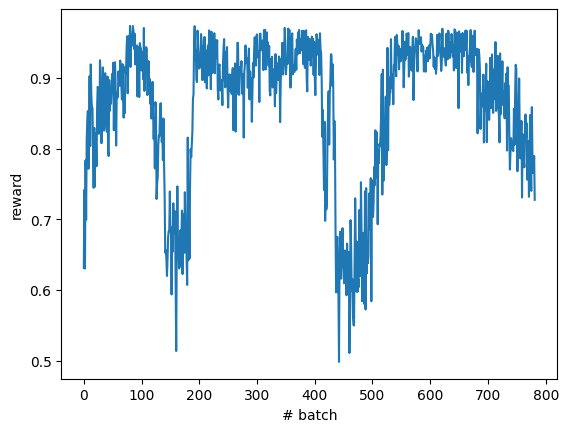
\includegraphics[]{q2.png}
      \caption{Reward over time.}
    \end{figure}
    
  \end{part}

  \begin{part}{\textbf{Provide $5$ example generations from the model. Are they
  more positive than the original generations? What else do you notice about
  them?}}

    Five example generations are:
    \begin{enumerate}
      \item ``\texttt{Young Elijah Wood and Joseph Mazzello are outstanding
      actors. I like this. I like this. I like this. I like this. I like}"
      \item ``\texttt{This is one of the best sequels around and a real
      classic,,,,,,,,,,,,,,,,,,}"
      \item ``\texttt{That's what me and my friends kept asking each other the
      most most most most most most most most most most most popular of most
      most most most most}"
      \item ``\texttt{"Mame" is a disgrace to many things. I like this. I like
      this. I like this. I like this. I like this}"
      \item ``\texttt{The Tender Hook, or, Who Killed The New York. I like this.
      I like this. I like this. I like this. I}"
    \end{enumerate}
    These generations are certainly more positive than the original generations,
    as they all contain the phrase ``I like this" or some other positive phrase
    repeated over and over again. This is likely because the model has learned
    that repeating positive phrases is likely to receive a high reward.

  \end{part}

  \begin{part}{\textbf{What are the limitations of REINFORCE based on your
  observations of the generated reviews? Explain what might have caused such
  limitations.}}

    The limitations of REINFORCE based on the observations of the generated
    reviews are that the model seems to be stuck in a loop of repeating the same
    words over and over again. This is probably because the model is not
    learning to generate coherent sentences, and is instead trying to generate
    sequences of words that maximize the reward.
    
    This is a limitation of REINFORCE because it doesn't take into account the
    structure of the generated sequences, and instead just tries to maximize the
    reward by generating sequences that are likely to receive high rewards. In
    this case, saying something like ``I like this" over and over again is
    likely to receive a high reward, so it is a valid strategy for the model to
    pursue.
  \end{part}

  \begin{part}{\textbf{What does \texttt{reset\_model\_optimizer} do?}}

    The \texttt{reset\_model\_optimizer} function initializes / resets the
    pre-trained causal LM and its optimizer for training. It sets the model's
    padding token ID to match the end-of-sentence token ID of the tokenizer, so
    that the sequences are processed correctly. Also, it initializes the
    optimizer to an AdamW optimizer with the given learning rate.

    It's basically just used to reset the model and optimizer to their initial
    states, so that we can train the model from scratch. This is useful when we
    want to train the model for multiple epochs, as we can reset the model and
    optimizer to their initial states after each epoch, so that we can train the
    model from scratch each time.
  \end{part}

  \begin{part}{\textbf{What's the shape of \texttt{log\_probs} in
  \texttt{compute\_reinforce\_loss}, and what does each dimension correspond
  to?}}

    The shape of \texttt{log\_probs} is \texttt{[batch\_size, sequence\_length,
    vocab\_size]}.

    In this case, the \texttt{batch\_size} is 32, the \texttt{sequence\_length}
    is 30, and the \texttt{vocab\_size} is 50257.

    The \texttt{batch\_size} dimension corresponds to the number of sequences in
    the batch, the \texttt{sequence\_length} dimension corresponds to the length
    of each sequence, and the \texttt{vocab\_size} dimension corresponds to the
    size of the vocabulary.
  \end{part}

\end{question}

\begin{question}{Regularization}

  \begin{part}{\textbf{First, run your REINFORCE training function with $\alpha
  = 0$ for $1$ epoch. This is equivalent to training without the KL-penalty.
  Plot the KL-divergence between the original model and the new model over time.
  What trend do you see from the plot? Why could such a trend be undesirable in
  practice?}}

    \begin{figure}[h]
      \centering
      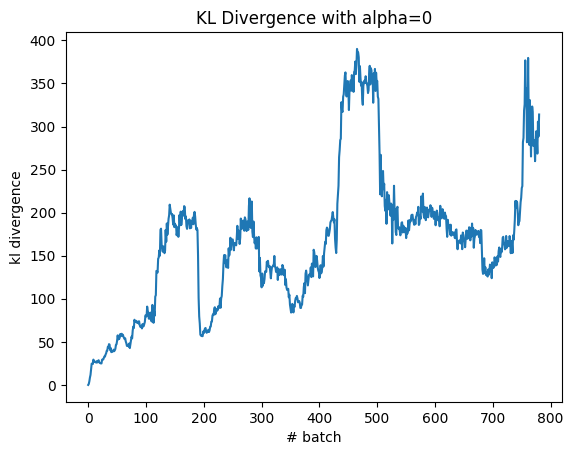
\includegraphics[]{q3part1.png}
      \caption{KL-divergence over time with $\alpha = 0$.}
    \end{figure}

    The trend I see from the plot is that the KL-divergence between the original
    model and the new model is increasing over time. This is undesirable in
    practice because it means that the new model is diverging from the original
    model, and is no longer a good approximation of the original model.
  \end{part}

  \begin{part}{\textbf{Try different $\alpha$ to experiment with the power of
    KL-regularization. For each setup, report the $\alpha$ values, the
    KL-divergence plots, reward plots, $5$ sample generations, and comments on
    the samples' quality.}}
    
    \textbf{A high $\alpha$ that prevents the model from being able to get a
    reward of $0.65$ or more.}

    I tried $\alpha = 1000$.

    \vspace{5cm}

    \begin{figure}[h]
      \centering
      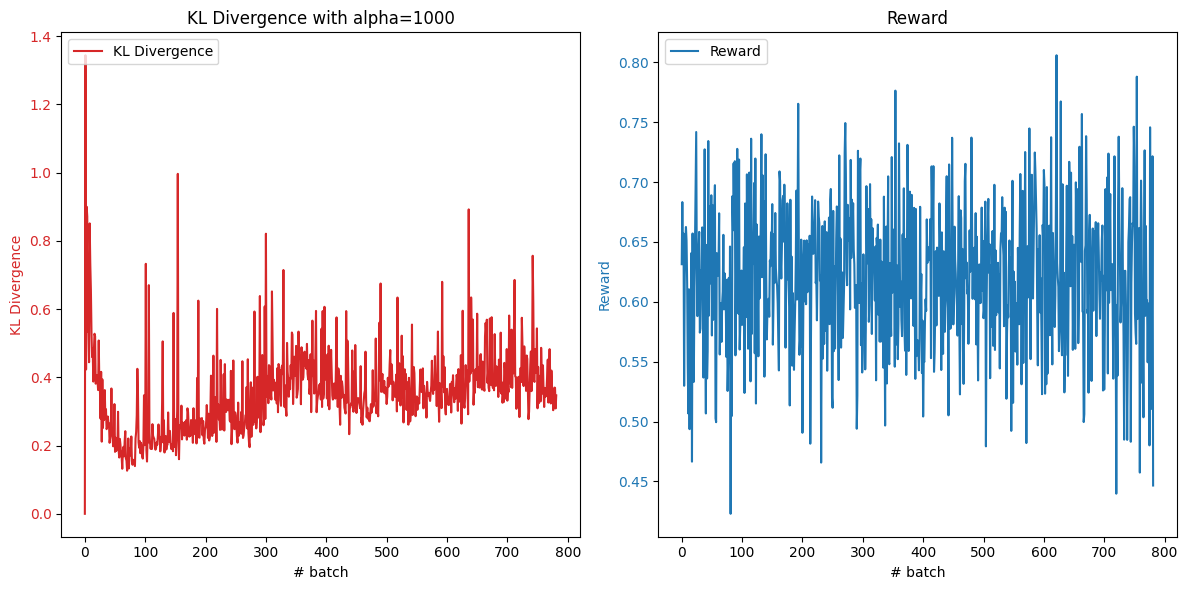
\includegraphics[scale=0.55]{q3alpha1000.png}
      \caption{KL-divergence and reward over time with $\alpha = 1000$.}
    \end{figure}

    Five example generations are:
    \begin{enumerate}
      \item ``\texttt{Young Elijah Wood and Joseph Mazzello are outstanding
      musicians and performers for the United States and the rest of the world.
      This was created in 1967 by}"
      \item ``\texttt{This is one of the best sequels around and a real star,
      just because they are better than many already.\textbackslash
      n\textbackslash n\textbackslash n\textbackslash nYou may see the}"
      \item ``\texttt{That's what me and my friends kept asking each other the
      day about. At one point, I asked if she'd take some of it away from}"
      \item ``\texttt{"Mame" is a disgrace to many things he did.\textbackslash
      n\textbackslash nP.S. I don't see the idea that this is a post}"
      \item ``\texttt{The Tender Hook, or, Who Killed The Tender Hook, or, Who
      Killed The Tender Hook, or, Who Killed the Tender}"
    \end{enumerate}

    The quality of the samples honestly looks like that in part 1. The $\alpha$
    value is way too high, and the model seems to overly regularize which leads
    it to not learn anything at all. The generations don't seem positive, they
    just seem like fragmented natural language follow-ups, which is probably
    because the regularization is so high. Because of this, the reward isn't as
    high either, just like in part 1 where the reward was also under 0.65. \\\\
    \textbf{A low $\alpha$ such that the outputs are poor quality.}
    I tried $\alpha = 1e8$.

    \begin{figure}[h]
      \centering
      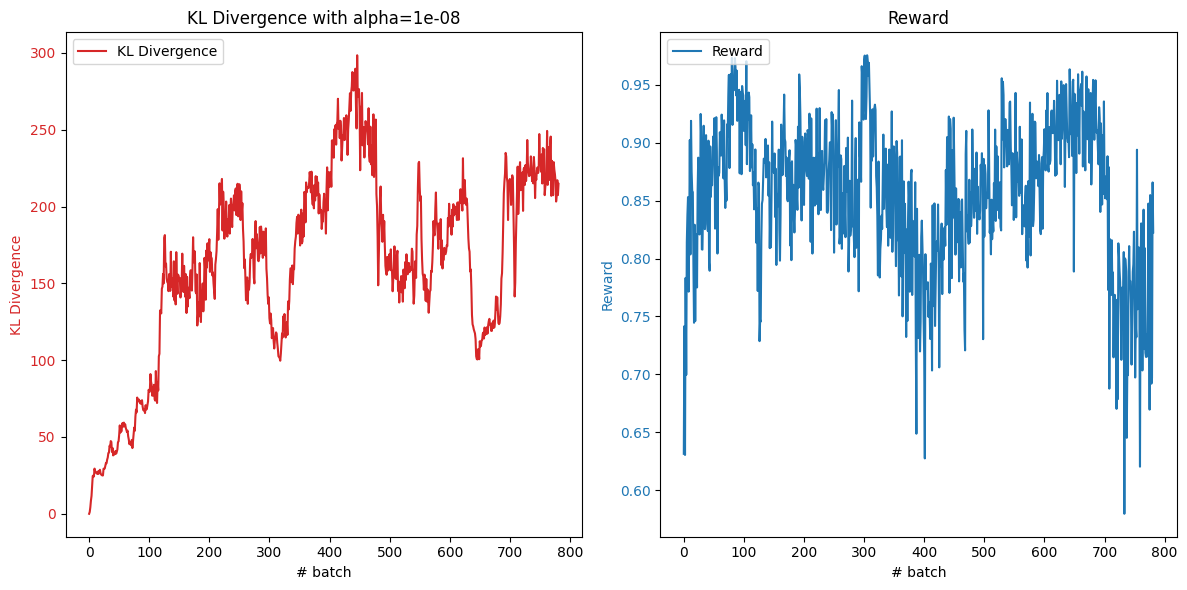
\includegraphics[scale=0.55]{q3alpha1e8.png}
      \caption{KL-divergence and reward over time with $\alpha = 1e8$.}
    \end{figure}

    Five example generations are:
    \begin{enumerate}
      \item ``\texttt{Young Elijah Wood and Joseph Mazzello are outstanding
      actors and I loved loved loved loved loved loved loved loved loved loved
      loved loved loved loved loved loved loved}"
      \item ``\texttt{This is one of the best sequels around and a very good
      movie. loved loved loved loved loved loved loved loved loved loved loved
      loved loved loved loved loved}"
      \item ``\texttt{That's what me and my friends kept asking each other the
      very very very very very very very very very very very very very very very
      very very very}"
      \item ``\texttt{"Mame" is a disgrace to many things he did in his life.
      loved loved loved loved loved loved loved loved loved loved loved loved
      loved loved}"
      \item ``\texttt{The Tender Hook, or, Who Killed The Tenders. loved loved
      loved loved loved loved loved loved loved loved loved loved loved loved
      loved loved loved}"
    \end{enumerate}

    The quality of the samples is very poor, as the model is just repeating the
    same words over and over again. This is likely because the $\alpha$ value is
    so low that the model is not being regularized at all, and is instead just
    trying to maximize the reward by generating sequences that are likely to
    receive high rewards.

    As discussed in part 2, this is the limitation behind REINFORCE, and it's
    clear that the model is just trying to maximize the reward by generating
    sequences (this time just words) that are likely to receive high rewards.
    \\\\
    \textbf{An $\alpha$ that gets a good reward ($\geq 0.8$) and outputs mostly
    natural text.}

    I chose $\alpha = 0.0003$.

    \begin{figure}[h]
      \centering
      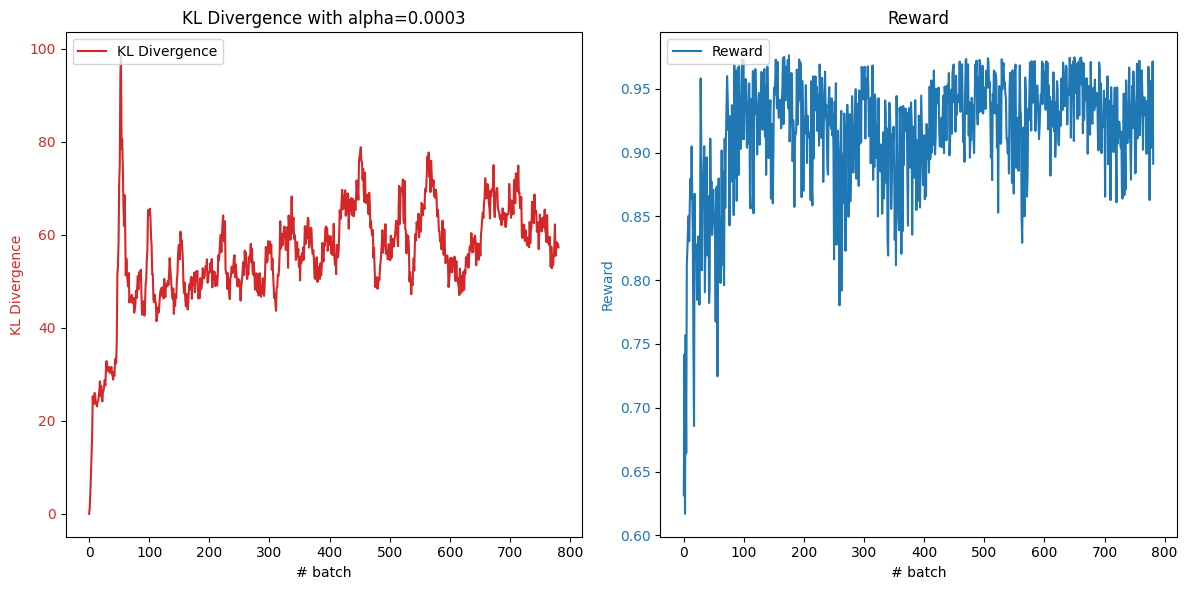
\includegraphics[scale=0.55]{q3alpha5e4.png}
      \caption{KL-divergence and reward over time with $\alpha = 0.0003$.}
    \end{figure}

    Five example generations are:
    \begin{enumerate}
      \item ``\texttt{Young Elijah Wood and Joseph Mazzello are outstanding
      actors and I am a great time to do a great things. I think it is a great
      time}"
      \item ``\texttt{This is one of the best sequels around and a real movie,
      it's a great time for us and I am a great time to feel this to}"
      \item ``\texttt{That's what me and my friends kept asking each other the
      time. I think it's wonderful. I'm a great young, and I'm happy}"
      \item ``\texttt{"Mame" is a disgrace to many things this movie is great
      and we are great with no regrets at all the time. If you are a}"
      \item ``\texttt{The Tender Hook, or, Who Killed The Tenders, and I think
      the best time to do a great things. But I'll be very}"
    \end{enumerate}

    The quality of these samples is better! It's not perfect, and doesn't really
    make sense, but at least it's natural language (even if it's not
    grammatically correct). Things like "I think it's wonderful" and "I think it
    is a great time" are positive, however it seems to have an obsession with
    talking about a "great time." This is probably because the regularization is
    not high enough, so maybe increasing $\alpha$ a bit would help, but overall
    the reward is solid and the KL-divergence stayed low, so it's a good
    balance.
  \end{part}

  \begin{part}{\textbf{Based on your experience with REINFORCE with
  KL-regularization, identify one of its main limitations and propose a
  potential solution. There’s no single right answer here; any justifiable
  answer will result in full credit.}}

    One issue with REINFORCE with KL-regularization is that it can be difficult
    to tune the $\alpha$ hyperparameter. If $\alpha$ is too high, the model will
    be overly regularized and will not learn anything at all. If $\alpha$ is too
    low, the model will not be regularized at all, and will instead just try to
    maximize the reward by generating sequences that are likely to receive high
    rewards.

    One potential solution to this issue is to use \textbf{annealing}.
    Basically, we start with a high value of $\alpha$ (high regularization) and
    then gradually decrease it over time. This can help to ensure that the model
    is regularized enough to prevent it from generating incoherent sequences,
    but is not overly regularized so that it cannot learn anything at all.

  \end{part}

  \begin{part}{\textbf{Over which tokens do we compute the REINFORCE loss, and
  why?}}

    We compute the REINFORCE loss over the tokens in the sequence themselves.
    This is because it allows us to take the gradient of the reward with respect
    to the model's parameters to favor sequences of tokens that lead to higher
    rewards. It's just basic gradient descent, but with the reward as the
    objective function. (Actually I guess in this case it's gradient ascent,
    since we're trying to maximize the reward.)

  \end{part}
  
\end{question}
\clearpage
\begin{question}{DPO Implementation}
  
  \begin{part}{\textbf{Run your training function for $2$ epochs using the batch
  size $16$. Plot the training losses over time and report the model’s average
  loss on the test set for the final model. Note that an efficient
  implementation should run in about $10$ minutes.}}

  The DPO test loss was $\boxed{0.5968}$.
  
    \vspace{5cm}
    \begin{figure}
      \centering
      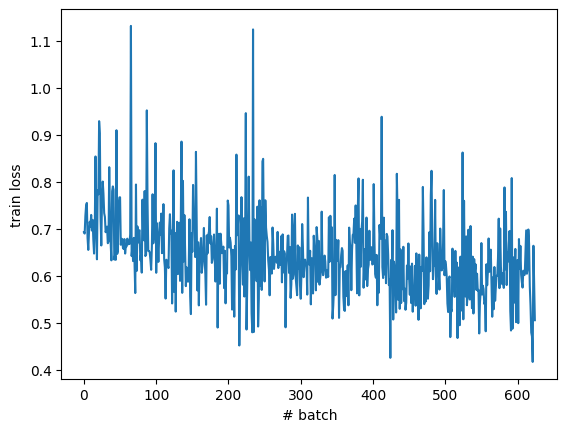
\includegraphics[]{dpo_loss.png}
      \caption{DPO training loss over time.}
    \end{figure}

  \end{part}

  \begin{part}{\textbf{Run the evaluation function using the same data and code
    from Section $1$ using the DPO-trained model. How does the reward compare to
    the REINFORCE model? Why do you think the results look like this?}}

    There are many reasons this could happen, from hyperparameter sensitivity to
    the fact that REINFORCE can do reward hacking to get a really high reward.
    It's also possible that the DPO model is just not learning as well as the
    REINFORCE model, or that the DPO model is overfitting to the training data.
  \end{part}

  \begin{part}{\textbf{Provide 5 example generations from the DPO-trained model.
  Are they more positive than the original generations? What else do you notice
  about them?}}

    Five example generations are:
    \begin{enumerate}
      \item ``\texttt{Young Elijah Wood and Joseph Mazzello are outstanding
      musicians and performers for the United States, the United Kingdom, the
      Netherlands, Turkey, and France.}"
      \item ``\texttt{This is one of the best sequels around and a real star,
      just because they are better than many others.\textbackslash
      n\textbackslash n\textbackslash n\textbackslash nYou may not know}"
      \item ``\texttt{That's what me and my friends kept asking each other the
      day about. At one point, I asked if she'd take some of it away from}"
      \item ``\texttt{"Mame" is a disgrace to many things he did.\textbackslash
      n\textbackslash nP.S. I don\'t actually like it too much...\textbackslash
      nM}"
      \item ``\texttt{The Tender Hook, or, Who Killed The Tender Hook, or, Who
      Killed The Tender Hook, or, Who Killed the Tender}"
    \end{enumerate}

    These generations are not more positive than the original generations, and
    are in fact basically the same as the original generations. This is likely
    because the DPO model is just overfitting to the training data, or is really
    sensitive to the hyperparameters (a likely outcome as I haven't tuned them).
    Compared to REINFORCE, which had really different generations (but
    reward-hacked generations), the DPO model seems to be generating more
    natural language, even though the sentence doesn't make much sense. But the
    sentiment is not really positive.

  \end{part}

  \begin{part}{\textbf{Try $3$ different values for $\beta$ (note it’s typically
  set to be in the range of $0.1$ to $0.5$). Plot the training loss plots and
  report the final test losses for each of these setups. What's the best setup
  that you found? How do different values of $\beta$ impact the training
  differently?}}
    
    I tried $\beta$ values of 0.1, 0.25, and 0.4.

    \begin{figure}[h]
      \centering
      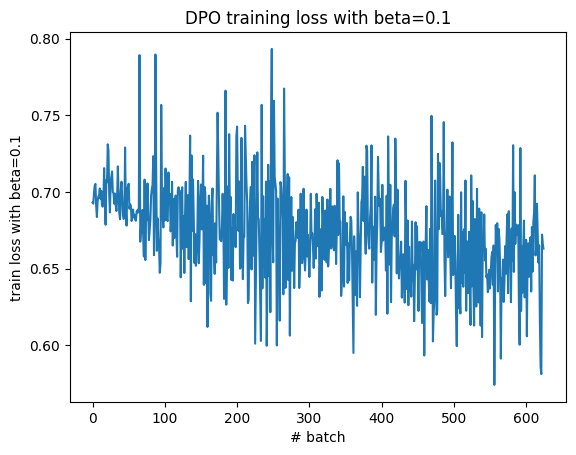
\includegraphics[scale=0.7]{q401.png}
      \caption{DPO training loss over time with $\beta = 0.1$.}
    \end{figure}

    The final test loss for $\beta = 0.1$ was $\boxed{0.6521}$ (best setup). 

    \begin{figure}[h]
      \centering
      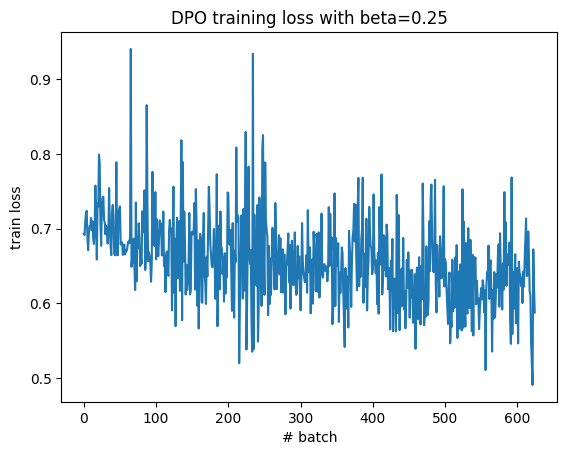
\includegraphics[scale=0.7]{q4025.png}
      \caption{DPO training loss over time with $\beta = 0.25$.}
    \end{figure}

    The final test loss for $\beta = 0.25$ was $\boxed{0.6207}$.

    \begin{figure}[h]
      \centering
      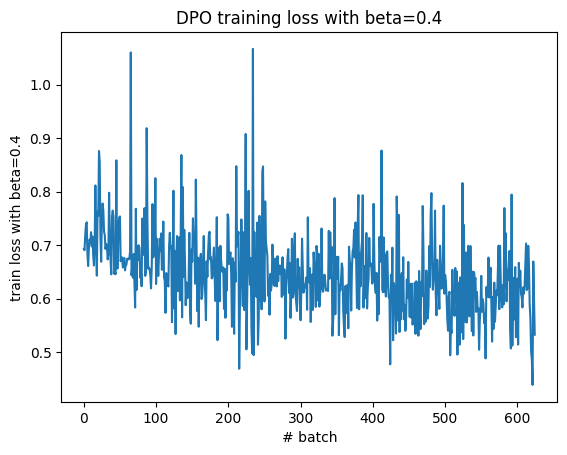
\includegraphics[scale=0.7]{q404.png}
      \caption{DPO training loss over time with $\beta = 0.4$.}
    \end{figure}

    The final test loss for $\beta = 0.4$ was $\boxed{0.6044}$.

    It seems that as $\beta$ increased, so did the test loss. The smaller values
    of $\beta$ seem to perform better.
  \end{part}
  \clearpage
  \begin{part}{\textbf{What’s the purpose of using $\sigma$, the logistic
  function, in $\mathcal{L}_{\text{DPO}}$?}}
    
    $\sigma$ is used to keep the output of the log probability ratios in the
    range $[0, 1]$. It also sort of smooths the output, so that the model can
    calculate gradients more easily.

  \end{part}

  \begin{part}{\textbf{What are the main differences and advantages of DPO
    compared to other online RL methods like PPO?}}
    
    DPO directly optimizes the policy, by increasing the likelihood of preferred
    actions and decreasing the likelihood of non-preferred actions. This is
    different from PPO, which uses a clipped objective function to prevent the
    policy from changing too much at each iteration.

    Because PPO has a clipping mechanism, beneficial updates can be discarded if
    they fall outside the clipping range.

    The logistic function in DPO provides smoother gradient updates as well (see
    above answer).

  \end{part}
  
\end{question}
\clearpage
\begin{question}{GPT-4 Capability Forecast}

  Large language models are surprisingly good at some things, and surprisingly
  bad at others. Test and build your intuition for GPT-4’s capabilities in this
  online quiz:
  https://nicholas.carlini.com/writing/llm-forecast/question/Capital-of-Paris
  
  \begin{part}{\textbf{Report your accuracy and log loss.}}
    \begin{itemize}
      \item \textbf{Accuracy}: 64.29\%
      \item \textbf{Average Log Loss}: 1.079
    \end{itemize}
    This abysmal performance on my part suggets that I have a soft side for
    GPT-4, as I was wildly overconfident in my guesses, and thus my confidence
    levels were not well-calibrated.
  \end{part}

  \begin{part}{\textbf{Was there anything you expected GPT-4 to be able to do
  that it couldn’t do? Or vice versa?}}

  I expected that GPT-4 would be able to answer certain questions like Password
  or Tic-Tac-Toe, but turns out these sorts of tasks are too complex or require
  logical reasoning that can't be handled.

  On the other hand, I was surprised that it could do math really well (like
  take an integral) and also the JavaScript code was really cool! Making an
  entire flag was very impressive and something that would take me a really long
  time.

  \end{part}

  \begin{part}{\textbf{What patterns do you notice in the failure/success modes?
    Can you guess the reasons behind these failure/success modes?}}
    
    I noticed that GPT-4 was really good at generating text that was similar to
    the training data, but was bad at other things. For example, it was really
    easy to emulate the style of a certain author, but it was really hard to
    answer questions that required logical reasoning.

    I guess the reasons for this are because GPT-4 (and language models) can
    mimic existing text really well, but actually forming a new idea (through
    logical reasoning) is not as easy, as there's no textual basis for it to
    draw from.

  \end{part}

  \begin{part}{\textbf{Do you trust GPT-4 to help you with a task more or less
  after taking the quiz?}}

    I trust GPT-4 less after taking the quiz. I was surprised at how bad it was
    at some things, and I think I would be more cautious about using it for
    tasks that require logical reasoning or understanding of the world.
    
  \end{part}

  \begin{part}{\textbf{Using your wildest imagination, what capabilities do you
    hope the future GPT-x will have? Why are they important to have? What are
    some prerequisites if these capabilities were to be achieved in the future
    GPT-x? Be creative, and there’s no single correct answer!}}

    I hope that future GPT-x models will be able to understand the world and
    reason about it. This is important because it would allow us to use GPT-x
    for a wide range of tasks, from answering questions to solving problems to
    generating new ideas.

    I feel like a prerequisite for this would be safety. We need to make sure
    that if such an advanced language model would exist, it would not be used
    for malicious purposes. We also need to make sure that it is not biased, and
    that it is able to understand and reason about the world in a way that is
    consistent with human values.
    
  \end{part}

\end{question}

\end{document}